\chapter{DNA Models}
\label{chap:dna}


\section{3SPN.2C}
\label{sec:dna_3spn2c}

The series of the 3SPN.x DNA models have been developed by de Pablo's group.
The 3SPN.2C model is the one for modeling sequence-dependent curvature of
double-stranded DNA (dsDNA).  Particularly, the model has been well-tuned to
reproduce both mechanical and geometrical properties, such as persistent length
and major/minor groove widths.

\subsection{Topology}
\label{subsec:dna_3spn2c_top}

In this model, each nucleotide is represented by three CG particles, P
(phosphate), S (sugar), and B (base), as shown in
Figure~\ref{fig:dna_3spn2c_top}.  B has four types: A (adenine), C (cytosine), G
(guanine), and T (thymine).  The CG particles are put at the center-of-mass of
each chemical moiety.

\begin{figure}[ht]
  \centering
  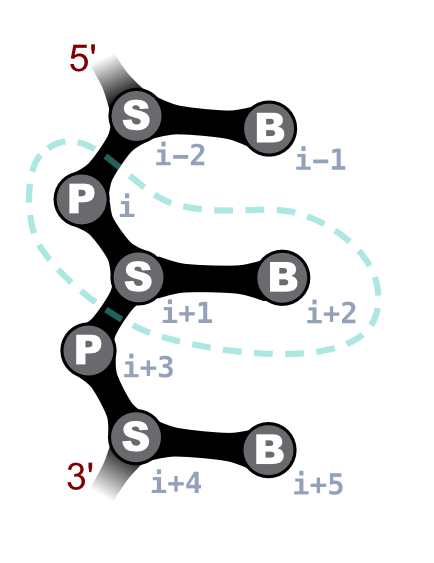
\includegraphics[width=0.3\textwidth]{figures/DNA_3spn2c_top.png}
  \caption{Topology of the 3SPN.2C DNA model: each nucleotide is represented by
    3 sites corresponding to phosphate (P), deoxyribose sugar (S), and
    nitrogenous base (B).  A typical nucleotide ``residue'' is enclosed by the
    dashed line.}
  \label{fig:dna_3spn2c_top}
\end{figure}


\begin{table}[ht]
  \centering
  \begin{tabular}{lc}
    \toprule
    Particle Type    & Mass (amu) \\
    \midrule
    P  &  94.97 \\
    S  &  83.11 \\
    A  &  134.1 \\
    C  &  110.1 \\
    G  &  150.1 \\
    T  &  125.1 \\
    \bottomrule
  \end{tabular}
  \caption{Mass of the 3SPN.2C DNA particles.}
  \label{tab:dna_3spn2c_top_mass}
\end{table}

\subsection{Potentials}
\label{subsec:dna_3spn2c_potential}

The 3SPN.2C potentials can be devided into two parts, as usual, bonded, and
nonbonded:
\begin{displaymath}
  U = U_b + U_{nb}.
\end{displaymath}

The bonded potentials include the following terms:
\begin{itemize}
\item bonds ($U_{bond}$),
\item angles ($U_{ang}$),
\item dihedral angles ($U_{dih}$).
\end{itemize}
\begin{equation}
  \label{eq:dna_3spn2c_local}
  U_b = U_{bond} + U_{ang} + U_{dih}.
\end{equation}

The nonbonded potentials include these terms:
\begin{itemize}
\item base-base interactions:
  \begin{itemize}
  \item base stacking ($U_{bstk}$),
  \item base pairing ($U_{bp}$),
  \item cross base stacking ($U_{cstk}$),
  \end{itemize}
\item excluded volume interactions ($U_{exv}$),
\item electrostatic interactions ($U_{ele}$).
\end{itemize}
\begin{equation}
  \label{eq:dna_3spn2c_nonlocal}
  U_{nb} = U_{bstk} + U_{bp} + U_{cstk} + U_{exv} + U_{ele}.
\end{equation}


\subsubsection{Bond}
\label{sec:dna_3spn2c_potential_bond}

\begin{smallpage}{3SPN.2C bond potential}<white>
  \begin{equation}
    \label{eq:dna_3spn2c_local_bond}
    U_{bond} = \sum_{i}^{bonds} k_b (r_i - r_{i,0})^2 + 100 k_b (r_i - r_{i,0})^4.
  \end{equation}
  \tcblower
  \begin{itemize}
  \item Bonds involved:
    \begin{itemize}
    \item P-S
    \item S-B
    \item S-P
    \end{itemize}
  \item $r_{i, 0}$: based on the structure of B-form DNA.
  \item $k_b = 0.6\ \mathrm{kJ/mol/\angstrom^2}$.
  \end{itemize}
\end{smallpage}



\subsubsection{Angle}
\label{sec:dna_3spn2c_potential_angle}

\begin{smallpage}{3SPN.2C bond angle potential}<white>
  \begin{equation}
    \label{eq:dna_3spn2c_local_angle}
    U_{ang} = \sum_{i}^{angles} k_\theta (\theta_i - \theta_{i,0})^2.
  \end{equation}
  \tcblower
  \begin{itemize}
  \item Angles involved:
    \begin{itemize}
    \item P-S-P
    \item S-P-S
    \item P-S-B
    \item B-S-P
    \end{itemize}
  \item $\theta_{i, 0}$: based on the structure of B-form DNA.
  \item $k_\theta$: see the table below: (unit: $\mathrm{kJ/mol/rad^2}$)
  \end{itemize}
  \begin{center}
    \begin{tabular}{l|cl|cl|cl|cl}
      \toprule
      \emph{PSP} & all & \multicolumn{7}{l}{300}\\
      \midrule
      \multirow{4}{*}{\emph{SPS}} &
                                    AA & 355 & AT & 147 & AC & 464 & AG & 368 \\
                 & TA & 230 & TT & 355 & TC & 442 & TG & 273 \\
                 & CA & 273 & CT & 368 & CC & 165 & CG & 478 \\
                 & GA & 442 & GT & 464 & GC & 228 & GG & 165 \\
      \midrule
      \multirow{4}{*}{\emph{PSB}} &
                                    AA & 460 & TA & 120 & CA & 206 & GA & 383 \\
                 & AT & 370 & TT & 460 & CT & 358 & GT & 442 \\
                 & AC & 442 & TC & 383 & CC & 278 & GC & 336 \\
                 & AG & 358 & TG & 206 & CG & 278 & GG & 278 \\
      \midrule
      \multirow{4}{*}{\emph{BSP}} &
                                    AA & 460 & AT & 370 & AC & 442 & AG & 358 \\
                 & TA & 120 & TT & 460 & TC & 383 & TG & 206 \\
                 & CA & 206 & CT & 358 & CC & 278 & CG & 278 \\
                 & GA & 383 & GT & 442 & GC & 336 & GG & 278 \\
      \bottomrule
    \end{tabular}
  \end{center}
\end{smallpage}

\subsubsection{Dihedral Angle}
\label{sec:dna_3spn2c_potential_dihedral_angle}

The dihedral angle potential in the 3SPN.2C model contains two parts:
\begin{enumerate}
\item A strong Gaussian type potential applied on the backbone dihedrals
  ($U_{dih, Gaussian}$);
\item A weak periodic potential applied on all dihedral angles ($U_{dih, periodic}$).
\end{enumerate}
\begin{equation}
  \label{eq:dna_3spn2c_local_dihedral}
  U_{dih} = U_{dih, Gaussian} + U_{dih, periodic}.
\end{equation}

\begin{smallpage}{3SPN.2C dihedral angle potential (Gaussian)}<white>
  \begin{equation}
    \label{eq:dna_3spn2c_local_dihedral_Gaussian}
    U_{dih, Gaussian} = \sum_{i}^{dihedrals} -k_{ \phi, Gaussian } \exp\big( \frac{-(\phi_i - \phi_{i,0})^2}{2\sigma_{\phi}^2} \big).
  \end{equation}
  \tcblower
  \begin{itemize}
  \item Dihedral angles involved:
    \begin{itemize}
    \item P-S-P-S
    \item S-P-S-P
    \end{itemize}
  \item $\phi_{i, 0}$: based on the structure of B-form DNA.
  \item $k_{\phi, Gaussian} = 7.0\ \mathrm{kJ/mol}$.
  \item $\sigma_\phi = 0.3\ \mathrm{rad^2}$.
  \end{itemize}
\end{smallpage}

\begin{smallpage}{3SPN.2C dihedral angle potential (periodic)}<white>
  \begin{equation}
    \label{eq:dna_3spn2c_local_dihedral_periodic}
    U_{dih, periodic} = k_{\phi, periodic} \big[ 1+\cos(\phi_i - \phi_{ i,0 }) \big].
  \end{equation}
  \tcblower
  \begin{itemize}
  \item Dihedral angles involved:
    \begin{itemize}
    \item P-S-P-S
    \item S-P-S-P
    \item S-P-S-B
    \item B-S-P-S
    \end{itemize}
  \item $\phi_{i, 0}$: based on the structure of B-form DNA.
  \item $k_{\phi, periodic} = 2.0\ \mathrm{kJ/mol}$.
  \end{itemize}
\end{smallpage}


\subsubsection{Base Stacking}
\label{sec:dna_3spn2c_potential_bstk}

Before we introduce the nonbonded terms, we would like to first show the
topology of the double stranded DNA and clarify the CG particles involved in the
base-base interaction terms (see Figure~\ref{fig:DNA_3spn2c_nonbonded_all}).

\begin{figure}[ht]
  \centering
  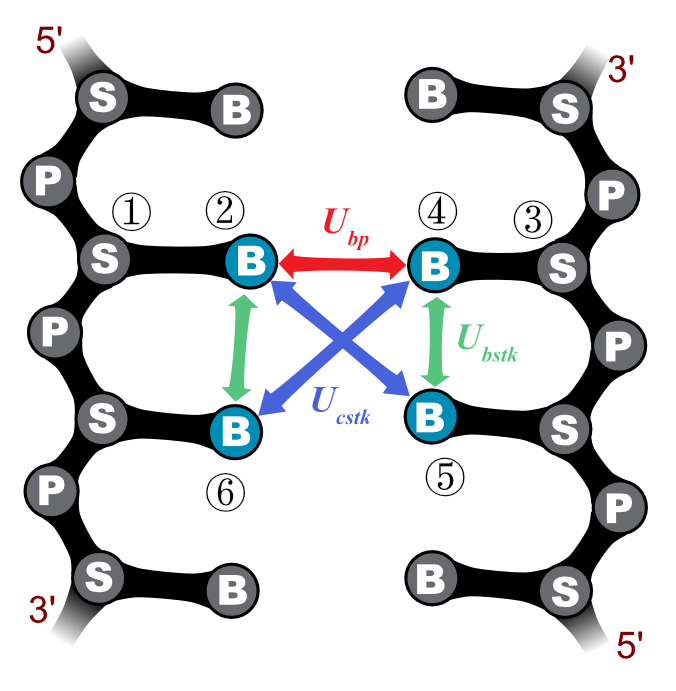
\includegraphics[width=0.45\textwidth]{figures/DNA_3spn2c_nonbonded_all.png}
  \caption{The base-related nonbonded interactions among DNA CG particles.  Here
    we introduce local indices (circled numbers) for easy understanding.  The
    base-stacking interactinos are calculated for the neighboring bases
    ($U_{bstk}$).  The base-pairing interactions are considered for Watson-Crick
    pairs, namely, the A-T and G-C pairs ($U_{bp}$).  Whereas the cross-stacking
    terms are only considered for bases next to the pairsing bases ($U_{cstk}$).}
  \label{fig:DNA_3spn2c_nonbonded_all}
\end{figure}

We would like to also define several common functions used by the
base-interaction potentials:
\begin{equation}
  \label{eq:dna_3spn2c_nonlocal_base_rep}
  U_m^{rep}(\epsilon_{ij}, \alpha_{ij}, r_{ij}) =
  \begin{cases}
    \epsilon_{ij} \Big( 1-e^{\big(-\alpha_{ij}(r_{ij}-r_{ij,0})\big)} \Big)^2 & r_{ij} < r_{ij, 0}, \\[.5em]
    0 & r_{ij} \ge r_{ij, 0}.
  \end{cases}
\end{equation}

\begin{equation}
  \label{eq:dna_3spn2c_nonlocal_base_attr}
  U_m^{attr}(\epsilon_{ij}, \alpha_{ij}, r_{ij}) =
  \begin{cases}
    -\epsilon_{ij} & r_{ij} < r_{ij, 0}, \\[.5em]
    \epsilon_{ij} \Big(1-e^{\big(-\alpha_{ij}(r_{ij}-r_{ij,0})\big)} \Big)^2 - \epsilon_{ij} & r_{ij} \ge r_{ij, 0}.
  \end{cases}
\end{equation}

In Equation~\ref{eq:dna_3spn2c_nonlocal_base_rep} and
\ref{eq:dna_3spn2c_nonlocal_base_attr}, $r_{ij}$ is the distance between
particle $i$ and $j$, whereas $\epsilon_{ij}$ and $\alpha_{ij}$ are sequence
dependent parameters.

\begin{equation}
  \label{eq:dna_3spn2c_nonlocal_base_angle_mod}
  f(K, \Delta \theta) =
  \begin{cases}
    1 & \displaystyle -\frac{\pi}{2K} < \Delta \theta < \frac{\pi}{2K}, \\[.7em]
    1 - \cos^2(K\Delta\theta) & \displaystyle -\frac{\pi}{K} < \Delta \theta < -\frac{\pi}{2K} \textrm{ or } \frac{\pi}{2K} < \Delta \theta < \frac{\pi}{K}, \\[.7em]
    0 & \displaystyle \Delta \theta < -\frac{\pi}{K} \textrm{ or }  \Delta \theta > \frac{\pi}{K}. \\
  \end{cases}
\end{equation}

The $\theta$ in Equation~\ref{eq:dna_3spn2c_nonlocal_base_angle_mod} has
different definitions in $U_{bstk}$, $U_{bp}$, and $U_{cstk}$.

For the base-stacking interactions, $\theta_{BS}$ is the angle formed by
\circled{1}-\circled{2}-\circled{6}
(Figure~\ref{fig:DNA_3spn2c_nonbonded_bstk}).

Practically, we treat the $U_{bstk}$ as a ``local'' potential, because all the
interactions can be determined by the topology, regardless of the conformation.
Besides, the order of magnitude of computational cost of $U_{bstk}$ is only
$\mathcal{O}(n)$, where $n$ is the number of basepairs in DNA.

\begin{figure}[ht]
  \centering
  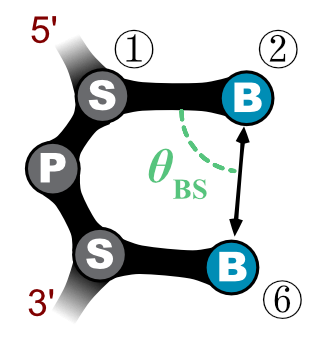
\includegraphics[width=0.2\textwidth]{figures/DNA_3spn2c_nonbonded_bstk.png}
  \caption{Definition of $\theta_{BS}$ in the base-stacking interactions.}
  \label{fig:DNA_3spn2c_nonbonded_bstk}
\end{figure}

\begin{smallpage}{3SPN.2C base-stacking potential}<white>
  \begin{equation}
    \label{eq:dna_3spn2c_nonlocal_base_stacking}
    U_{bstk} = \sum^{n_{bstk}} U_m^{rep}(\epsilon_{BS, ij}, \alpha_{BS}, r_{ij}) +
    f(K_{BS}, \Delta\theta_{BS})
    U_m^{attr} (\epsilon_{BS, ij}, \alpha_{BS}, r_{ij}).
  \end{equation}
  \tcblower
  \begin{itemize}
  \item Particles involved (see Figure~\ref{fig:DNA_3spn2c_nonbonded_bstk}):
    \begin{itemize}
    \item $r_{ij}$: \circled{2}-\circled{6}
    \item $\theta_{BS}$: \circled{1}-\circled{2}-\circled{6}
    \end{itemize}
  \item $\alpha_{BS} = 3.0$.
  \item $K_{BS} = 6.0$.
  \item $\epsilon_{BS, ij}$, $r_{ij, 0}$, and $\theta_{BS, 0}$: see the table below:
  \end{itemize}
  \begin{center}
    \begin{footnotesize}
      \begin{tabular}{ll|rrrr|rrrr|rrrr}
        \toprule
        & &  \multicolumn{12}{c}{\circled{6}}\\
        & & A & T & G & C & A & T & G & C & A & T & G & C \\
        \midrule
        & &  \multicolumn{4}{c|}{$\epsilon_{BS, ij}$ (kJ/mol)} & \multicolumn{4}{c|}{$r_{ij, 0}$ (\angstrom)} & \multicolumn{4}{c}{$\theta_{BS, 0}$ ($^\circ$)}\\
        \multirow{4}{*}{\circled{2}}
        & A & 13.82 & 15.05 & 13.32 & 15.82 & 3.58 & 3.56 & 3.85 & 3.45 & 100.13 & 90.48 & 104.39 &  93.23  \\
        & T &  9.15 & 12.44 &  9.58 & 13.11 & 4.15 & 3.93 & 4.32 & 3.87 & 102.59 & 93.32 & 103.70 &  94.55  \\
        & G & 13.76 & 14.59 & 14.77 & 15.17 & 3.51 & 3.47 & 3.67 & 3.42 &  95.45 & 87.63 & 106.36 &  83.12  \\
        & C &  9.25 & 12.42 &  8.83 & 14.01 & 4.15 & 3.99 & 4.34 & 3.84 & 102.69 & 96.05 & 100.46 & 100.68 \\
        \bottomrule
      \end{tabular}
    \end{footnotesize}
  \end{center}
\end{smallpage}



\subsubsection{Base Pairing and Cross-Stacking}
\label{sec:dna_3spn2c_potential_bp_cstk}

It is convenient to consider the $U_{bp}$ and $U_{cstk}$ potentials at the same
time, since $U_{cstk}$ only applies to bases next to the pairsing bases.  There
are also several angles and dihedral angles involved in the calculation of these
potentials (Figure~\ref{fig:DNA_3spn2c_nonbonded_bp_cstk}).


\begin{figure}[ht]
  \centering
  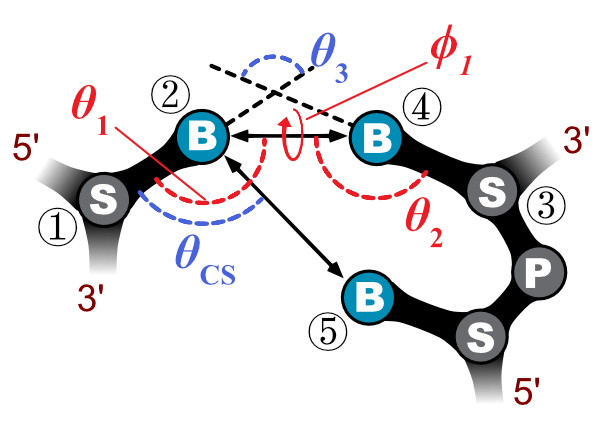
\includegraphics[width=0.4\textwidth]{figures/DNA_3spn2c_nonbonded_bp_cstk.png}
  \caption{Angles and dihedral angles involved in the $U_{bp}$ (red terms) and
    $U_{cstk}$ (blue terms) calculations.}
  \label{fig:DNA_3spn2c_nonbonded_bp_cstk}
\end{figure}

Note that the base pairsing interactions are considered when two bases satisfy
the following conditions:
\begin{itemize}
\item Base types can form Watson-Crick pairs: A-T, T-A, C-G, or G-C;
\item Base indices $i$ and $j$ are ``nonlocal'':
  \begin{itemize}
  \item $i$ and $j$ are in different strands;
  \item $i$ and $j$ are in the same strand, but $| i - j | > 10$.
  \end{itemize}
\end{itemize}


\begin{smallpage}{3SPN.2C base-pairing and cross-stacking potential}<white>
  \vspace{-1em}
  \begin{align}
    U_{bp} &= \sum^{n_{bp}} U_m^{rep}(\epsilon_{BP, ij}, \alpha_{BP}, r_{ij}) \nonumber \\
           &+ \frac{1}{2} \big( 1+\cos(\Delta \phi_1) \big)
             f(K_{BP}, \Delta\theta_{1})
             f(K_{BP}, \Delta\theta_{2})
             U_m^{attr} (\epsilon_{BP, ij}, \alpha_{BP}, r_{ij}).
             \label{eq:dna_3spn2c_nonlocal_base_pairing} \\[.5em]
    U_{cstk} &= \sum^{n_{cstk}} f(K_{BP}, \Delta\theta_{3})
               f(K_{CS}, \Delta\theta_{CS})
               U_m^{attr} (\epsilon_{CS, kl}, \alpha_{CS}, r_{kl}).
               \label{eq:dna_3spn2c_nonlocal_cross_stacking}
  \end{align}
  \tcblower
  \begin{itemize}
  \item Particles involved (see Figure~\ref{fig:DNA_3spn2c_nonbonded_bp_cstk}):
    \begin{itemize}
    \item $r_{ij}$: \circled{2}-\circled{4}
    \item $r_{kl}$: \circled{2}-\circled{5} and \circled{4}-\circled{6}, if available
    \item $\theta_{1}$: \circled{1}-\circled{2}-\circled{4}
    \item $\theta_{2}$: \circled{3}-\circled{4}-\circled{2}
    \item $\theta_{3}$: angle between vectors conecting \circled{1}-\circled{2} and \circled{3}-\circled{4}
    \item $\phi_{1}$: dihedral angle \circled{1}-\circled{2}-\circled{4}-\circled{3}
    \item $\theta_{CS}$: \circled{1}-\circled{2}-\circled{5} or \circled{3}-\circled{4}-\circled{6}
    \end{itemize}
  \item $\alpha_{BP} = 2.0$.
  \item $K_{BP} = 12.0$.
  \item $\alpha_{CS} = 4.0$.
  \item $K_{CS} = 8.0$.
  \item All the other parameters are listed in the table below:
  \end{itemize}
  \begin{center}
    \begin{footnotesize}
      \begin{tabular}{l|rrrrrr}
        \toprule
        \circled{2}-\circled{4} & $\theta_{1, 0}$ ($^\circ$) & $\theta_{2, 0}$  ($^\circ$) & $\theta_{3, 0}$  ($^\circ$) & $\phi_{1, 0}$  ($^\circ$) & $r_{ij, 0}$ ($\angstrom$) & $\epsilon_{BP, ij}$ (kJ/mol) \\
        \midrule
        A-T & 153.17 & 133.51 & 110.92 & -38.18 & 5.82 & 14.41 \\
        T-A & 133.51 & 153.17 & 110.92 & -38.18 & 5.82 & 14.41 \\
        G-C & 159.50 & 138.08 & 120.45 & -35.75 & 5.52 & 18.24 \\
        C-G & 138.08 & 159.50 & 120.45 & -35.75 & 5.52 & 18.24 \\
        \bottomrule
      \end{tabular}
    \end{footnotesize}
  \end{center}

  \begin{center}
    \begin{footnotesize}
      \begin{tabular}{ll|rrrr|rrrr|rrrr}
        \toprule
        & &  \multicolumn{12}{c}{\circled{5}}\\
        & & A & T & G & C & A & T & G & C & A & T & G & C \\
        \midrule
        & &  \multicolumn{4}{c|}{$\epsilon_{CS, kl}$ (kJ/mol)} & \multicolumn{4}{c|}{$r_{kl, 0}$ (\angstrom)} & \multicolumn{4}{c}{$\theta_{CS, 0}$ ($^\circ$)}\\
        \multirow{4}{*}{\circled{2}}
        & A & 1.882 & 2.388 & 2.439 & 1.680 & 6.42 & 6.77 & 6.27 & 6.84 & 154.04 & 158.77 & 153.88 & 157.69 \\
        & T & 2.388 & 1.882 & 2.187 & 2.566 & 6.77 & 7.21 & 6.53 & 7.08 & 148.62 & 155.05 & 147.54 & 153.61 \\
        & G & 2.439 & 2.187 & 3.250 & 0.972 & 6.27 & 6.53 & 5.74 & 6.86 & 153.91 & 155.72 & 151.84 & 157.80 \\
        & C & 1.680 & 2.566 & 0.972 & 4.135 & 6.84 & 7.08 & 6.86 & 6.79 & 152.04 & 157.72 & 151.65 & 154.49 \\
        \bottomrule
      \end{tabular}
    \end{footnotesize}
  \end{center}

  \begin{center}
    \begin{footnotesize}
      \begin{tabular}{ll|rrrr|rrrr|rrrr}
        \toprule
        & &  \multicolumn{12}{c}{\circled{6}}\\
        & & A & T & G & C & A & T & G & C & A & T & G & C \\
        \midrule
        & &  \multicolumn{4}{c|}{$\epsilon_{CS, kl}$ (kJ/mol)} & \multicolumn{4}{c|}{$r_{ij, 0}$ (\angstrom)} & \multicolumn{4}{c}{$\theta_{CS, 0}$ ($^\circ$)}\\
        \multirow{4}{*}{\circled{4}}
        & A & 1.882 & 2.388 & 2.566 & 2.187 & 5.58 & 6.14 & 5.63 & 6.18 & 116.34 & 119.61 & 115.19 & 120.92 \\
        & T & 2.388 & 1.882 & 1.680 & 2.439 & 6.14 & 6.80 & 6.07 & 6.64 & 107.40 & 110.76 & 106.33 & 111.57 \\
        & G & 2.566 & 1.680 & 4.135 & 0.972 & 5.63 & 6.07 & 5.87 & 5.66 & 121.61 & 124.92 & 120.52 & 124.88 \\
        & C & 2.187 & 2.439 & 0.972 & 3.250 & 6.18 & 6.64 & 5.66 & 6.80 & 112.45 & 115.43 & 110.51 & 115.80 \\
        \bottomrule
      \end{tabular}
    \end{footnotesize}
  \end{center}
\end{smallpage}




\subsubsection{Excluded-Volume Interactions}
\label{sec:dna_3spn2c_potential_exv}


\begin{smallpage}{3SPN.2C excluded volume interaction}<white>
  \begin{equation}
    \label{eq:dna_3spn2c_nonlocal_exv}
    U_{exv} = \sum_{i<j}
    \begin{cases}\displaystyle
      \epsilon_r\bigg[ \Big(\frac{\sigma_{ij}}{r_{ij}} \Big)^{12} - 2 \Big(\frac{\sigma_{ij}}{r_{ij}} \Big)^6 \bigg]+ \epsilon_r & r < \sigma_{ij},  \\
      0 & r > \sigma_{ij}.
    \end{cases}
  \end{equation}
  \tcblower
  \begin{itemize}
  \item $i, j$ are all pairs of CG particles that are \emph{not} in the
    following list:
    \begin{itemize}
    \item bonded (involved in bonds, angles, or dihedrals);
    \item particles in the neighboring nucleotides;
    \item Watson-Crick base pairs.
    \end{itemize}
  \item $\epsilon_{r} = 1.0$ kJ/mol.
  \item $\displaystyle \sigma_{ij} = \frac{1}{2}\big( \sigma_i + \sigma_j
    \big)$, where $\sigma_i$ ($\sigma_j$) is listed below:
  \end{itemize}
  \begin{center}
    \begin{tabular}{lc}
      \toprule
      Particle Type    & $\sigma$ ($\angstrom$) \\
      \midrule
      P  &  4.5 \\
      S  &  6.2 \\
      A  &  5.4 \\
      C  &  6.4 \\
      G  &  4.9 \\
      T  &  7.1 \\
      \bottomrule
    \end{tabular}
  \end{center}
\end{smallpage}
